The assignment was to improve the implementation from the previous exercise with
a pipeline instead of the datapath, and implement optimizations that improve the
performance of the processor. This was to be tested on the FPGA onboard a 
MicroBlaze-based embedded system.

\subsection{Requirements}
The processor should include a 5-stage pipeline, and otherwise follow the
requirements from the previous exercise. This includes using a limited MIPS
instruction set.

\subsection{Suggestions}
It was suggested that we followed the architecture presented by Patterson and
Hennessy, as supplied in figure \ref{fig:suggestedArchitecture}.

\begin{figure}[ht]
    \centering
    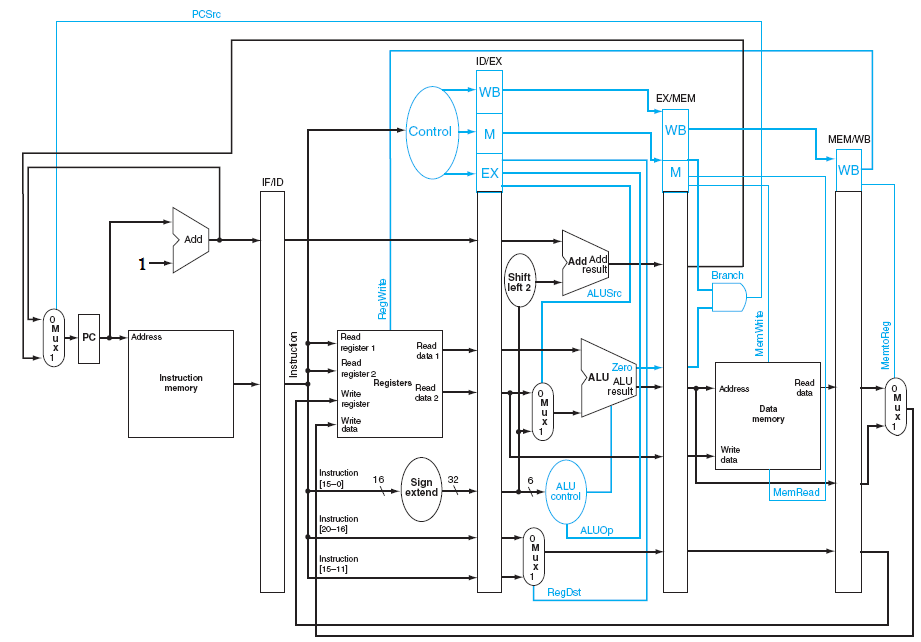
\includegraphics[width=\textwidth]{figures/SuggestedArchitecture.png}
    \caption{The suggested CPU architecture} 
    \label{fig:suggestedArchitecture}
\end{figure}


\subsection{Supplied material}
\begin{itemize}
    \item Communication Framework -  Providing an interface towards the embedded system
    \item VHDL Components - Register File, ALU and Adder
    \item Test Program - For verification of design
    \item main.c - MicroBlaze script for handling communication
    \item host.py - Python script for handling communication
\end{itemize}
